\documentclass[11pt,aspectratio=169]{beamer}

\usepackage{slides}
\usepackage{soul}
\usepackage{pdfpc}
\usepackage{ebproof}
\usepackage{bigdelim}
\usepackage{booktabs}
\usepackage{listings}
\usepackage{tcolorbox}
\usepackage{tabularx}
\usepackage{tikz}
\usepackage{xspace}
\usepackage[T1]{fontenc}
\usepackage[utf8]{inputenc}
\usepackage[symbol]{footmisc}
\usepackage[noend]{algpseudocode}
\usepackage[
    backend    = biber,
    style      = alphabetic,
    giveninits = true,
    maxnames   = 16,
    minnames   = 16,
]{biblatex}

\addbibresource{./references.bib}

\usetikzlibrary{
    positioning,
    shapes.symbols,
    shadows,
    arrows,
    calc
}

\newcommand{\senc}{\text{senc}}
\newcommand{\msg}{\text{msg}}
\newcommand{\nonce}{\text{nonce}}
\newcommand{\KDF}{\text{KDF}}
\newcommand{\key}{\text{key}}

\newcommand{\Tamarin}[1]{\textsc{Tamarin}\xspace}

%% Print: [#1] -[#2]-> [#3]
\newcommand{\MSR}[3]{#1 -\hspace{-4pt}[\hspace{5pt} #2 \hspace{4pt}]\hspace{-4.6pt}\rightarrow #3}
%% Print: -[#1]->
\newcommand{\ActionFact}[1]{-\hspace{-4pt}[\hspace{5pt} #1 \hspace{4pt}]\hspace{-4.6pt}\rightarrow}
%% Print: ~
\newcommand{\tildelow}{\raisebox{0.5ex}{\texttildelow}}
%% Print: ^
\newcommand{\pow}{\textasciicircum{}}
%% Highlight text in overlay
\newcommand{\althl}[2][2]{\alt<#1>{\hl{#2}}{#2}}

%% Sticky notes to represent facts
\definecolor{StickyNoteYellow}{RGB}{241,239,161}
\definecolor{StickyNoteRed}{RGB}{255,167,169}
\definecolor{StickyNoteGreen}{RGB}{148,199,146}
\definecolor{StickyNoteBlue}{RGB}{167,229,241}
\NewDocumentCommand{\StickyNote}{O{StickyNoteYellow}O{1cm}m}{%
    \begin{tikzpicture}
        \node[
            drop shadow={
                shadow xshift = 2pt,
                shadow yshift = -4pt,
            },
            xslant = -0.1,
            yslant = 0.1,
            draw   = black,
            fill   = #1,
            text   = black,
        ] {\parbox[t][#2][c]{#2}{\centering#3}};
    \end{tikzpicture}
}

%% Colors for terms and facts
\definecolor{TermBlue}{HTML}{1C377D}
\definecolor{FactPurple}{HTML}{7C3655}

\newcommand{\term}[1]{\textcolor{TermBlue}{#1}}
\newcommand{\Term}[1]{\textcolor{TermBlue}{#1}}
\newcommand{\Fact}[1]{\textcolor{FactPurple}{#1}}

%% Other colors
\definecolor{AdversaryRed}{HTML}{DA3B26}

%% Listings
\lstset{escapeinside={(*@}{@*)}}
\lstset{numberstyle=\tiny}

\definecolor{TamarinBlue}{RGB}{42,0,255}
\definecolor{TamarinGreen}{RGB}{48,110,32}
\definecolor{TamarinPurple}{RGB}{175,36,67}

\lstdefinestyle{tamarin}{
    basicstyle    = \linespread{0.75}\footnotesize\ttfamily,
    extendedchars = true,
    tabsize       = 2,
    columns       = fixed,
    numbers       = none,
    breaklines    = true,
    literate      = {~}{{\raisebox{0.5ex}{\texttildelow}}}{1},
    morekeywords  = {theory, builtins, restriction, equations, functions, rule,
                     let, in, lemma, All, Ex, not, predicates, begin, end},
    keywordstyle  = \color{TamarinPurple},
    morecomment   = [l]{//},
    morecomment   = [s]{/*}{*/},
    commentstyle  = \color{TamarinGreen},
    xleftmargin   = 0mm,
    upquote       = true,
    morestring    = *[b]",
    showstringspaces = false
}

\lstdefinestyle{tactic}{
    basicstyle    = \linespread{0.75}\footnotesize\ttfamily,
    extendedchars = true,
    tabsize       = 2,
    columns       = fixed,
    numbers       = none,
    breaklines    = true,
    literate      = {~}{{\raisebox{0.5ex}{\texttildelow}}}{1},
    alsoletter    = :,
    morekeywords  = {tactic:, presort:, prio:, deprio:},
    keywordstyle  = \color{TamarinPurple},
    morecomment   = [l]{//},
    morecomment   = [s]{/*}{*/},
    commentstyle  = \color{TamarinGreen},
    xleftmargin   = 0mm,
    upquote       = true,
    morestring    = *[b]",
}

\lstdefinestyle{oracle}{
    basicstyle    = \linespread{0.75}\footnotesize\ttfamily,
    extendedchars = true,
    tabsize       = 2,
    columns       = fixed,
    numbers       = none,
    breaklines    = true,
    literate      = {~}{{\raisebox{0.5ex}{\texttildelow}}}{1},
    morecomment   = [l]{\#},
    morekeywords  = {import, for, in, if, elif},
    keywordstyle  = \color{TamarinPurple},
    commentstyle  = \color{TamarinGreen},
    xleftmargin   = 0mm,
    upquote       = true,
}

\definecolor{ProVerifGreen}{RGB}{48,110,32}
\definecolor{ProVerifBlue}{RGB}{64,112,161}

\lstdefinestyle{proverif}{
    basicstyle    = \linespread{0.75}\footnotesize\ttfamily,
    extendedchars = true,
    tabsize       = 2,
    columns       = fixed,
    numbers       = none,
    breaklines    = true,
    literate      = {~}{{\raisebox{0.5ex}{\texttildelow}}}{1},
    morecomment   = [s]{(*}{*)},
    commentstyle  = \color{ProVerifGreen},
    keywordstyle  = \color{ProVerifBlue},
    morekeywords  = {in, if, event, new, let, out},
    xleftmargin   = 0mm,
}

\definecolor{proofTreeBlue}{HTML}{2639B0}
\definecolor{proofTreeRed}{HTML}{921C12}

\lstdefinestyle{prooftree}{
    basicstyle    = \linespread{0.8}\footnotesize\fontfamily{pcr}\selectfont,
    extendedchars = true,
    tabsize       = 2,
    columns       = fixed,
    numbers       = left,
    breaklines    = true,
    literate      = {~}{{\raisebox{0.5ex}{\texttildelow}}}{1},
    keywords      = [1]{lemma, case, next, qed, by, end, Diff-Lemmas},
    keywordstyle  = [1]\color{black}\bfseries,
    keywords      = [2]{simplify, solve, sorry, contradiction, induction,
                        autoprove, rule-equivalence},
    keywordstyle  = [2]\color{proofTreeBlue}\bfseries,
    keywords      = [3]{@, \|, <, \^},
    keywordstyle  = [3]\color{proofTreeRed},
    alsoletter    = @\|<\^-,
    moredelim     = **[is][{\color{proofTreeBlue}}]{<<}{>>},
    xleftmargin   = 0mm,
    upquote       = true,
    morestring    = *[b]",
}

%% Color boxes
\definecolor{ColorBoxBlue}{HTML}{1C377D}
\tcbset{
    colback      = white,
    colframe     = black,
    fonttitle    = \bfseries,
    coltitle     = white,
    colbacktitle = ColorBoxBlue,
    boxrule      = 1pt
}

%% Vertical separator for frames
\newcommand<>{\vsep}{
    \begin{tikzpicture}[remember picture,overlay]%
        \draw[ultra thick]
            ($(current page.north west)+(8cm,0.5cm)$) to
            ($(current page.south west)+(8cm,-0.5cm)$)
        ;
    \end{tikzpicture}%
}

%% Horizontal separator for frames
\newcommand<>{\hsep}{
    \begin{tikzpicture}[remember picture,overlay]%
        \draw[ultra thick]
            ($(current page.north west)+(-0.5cm,-4.5cm)$) to
            ($(current page.north east)+(0.5cm,-4.5cm)$)
        ;
    \end{tikzpicture}%
}


\title{Formal Analysis of Real-World Security Protocols}
\subtitle{Lecture 8: Advanced Features (Part 1)}
\date{\today}
\author{Aleksi Peltonen}
\institute{CISPA Helmholtz Center for Information Security}

\begin{document}
\maketitle

% ---------------------------------------------------------------------------- %
% Content
% ---------------------------------------------------------------------------- %

\begin{frame}[fragile]{Recap: Tamarin workflow}
    \begin{figure}
        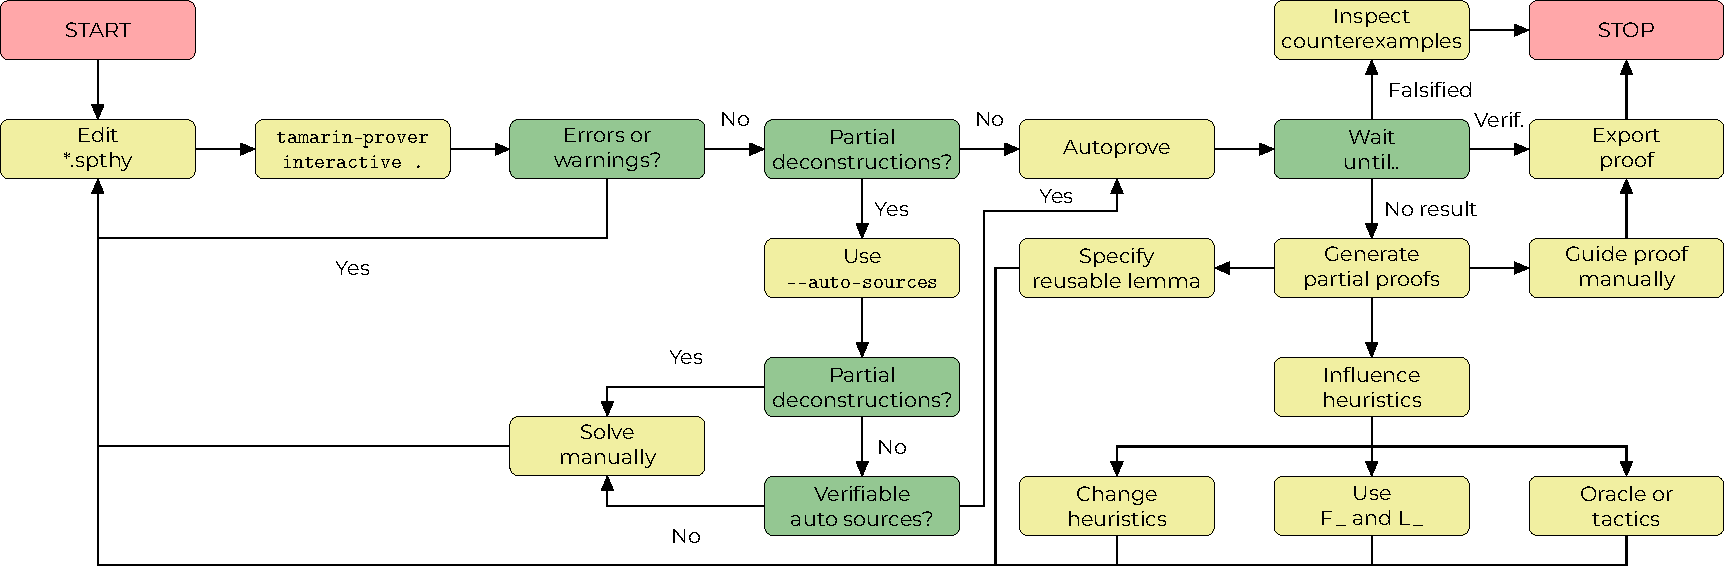
\includegraphics[width=\textwidth]{./figures/lecture_9/workflow_gui}
    \end{figure}
\end{frame}

\begin{frame}[fragile]{This lecture}
    \tableofcontents
\end{frame}

% ---------------------------------------------------------------------------- %

\section{Pre-Computation and Partial Deconstructions}

% ---------------------------------------------------------------------------- %

\begin{frame}[fragile]{Pre-computing sources}
    \begin{itemize}
        \item Tamarin performs optimizations to accelerate proof construction, 
              one of which is \textbf{pre-computation of sources}
        \item For all facts in the model: Backwards search with the constraint 
              solving algorithm to determine their sources
        \begin{itemize}
            \item Sources: \textbf{Partial executions} that yield a fact
            \item The search is incomplete; we do not check for non-termination
        \end{itemize}
        \item For \textbf{attacker knowledge}, Tamarin considers three cases:
        \begin{enumerate}
            \item Fresh values: \texttt{KU(\tildelow{}x)}
            \item Public values: \texttt{KU(\$x)}
            \item Function applications for all equations in the theory:
                  \texttt{KU(f($\mathrm{x_1, \dots, x_n}$))}
        \end{enumerate}
    \end{itemize}
\end{frame}

\begin{frame}[fragile]{Saturation}
    \begin{itemize}
        \item Once the pre-computation of sources is completed, Tamarin applies 
              a \textbf{saturation process}
        \begin{itemize}
            \item If there is an open premise inside a source corresponding to 
                  another source, the second source is applied to the open 
                  premise
            \item This is applied repeatedly until a fixpoint is reached or a 
                  bound is hit
        \end{itemize}
        \item Often fast, but can be limited \textbf{if necessary}
        \begin{itemize}
            \item Limit max number of saturations: \verb|--saturation=|
            \item Limit chain goals to solve: \verb|--open-chains=|
            \item Exclude facts from the pre-computations: \verb|[no_precomp]|
        \end{itemize}
        \item Use with caution; worth trying if Tamarin seems to be stuck in a
              loop
    \end{itemize}
\end{frame}

\begin{frame}[fragile]{Partial deconstructions}
    \begin{itemize}
        \item To avoid non-termination, Tamarin stops when it encounters a 
              chain goal that it cannot entirely resolve
        \begin{itemize}
            \item This is called a \textbf{partial construction}
                  (or an \textbf{open chain})
            \item Unresolved partial deconstructions often lead to
                  \textbf{non-termination when proving lemmas}
        \end{itemize}
        \item You can see a list of partial deconstructions in the GUI
    \end{itemize}
    \begin{center}
        \begin{tabular}{|l|}
            \hline
            \texttt{\textcolor[HTML]{2639B0}{
                Raw sources (9 cases, 6 partial deconstructions left)}}\\
            \texttt{\textcolor[HTML]{2639B0}{
                Refined sources (9 cases, deconstructions complete)}}\\
            \hline
        \end{tabular}
    \end{center}
    \begin{itemize}
        \item The command-line interface will \textbf{not show you these}
    \end{itemize}
\end{frame}

\begin{frame}[fragile]{Sources lemmas}
    \begin{itemize}
        \item Tamarin's internal pre-computations can be inspected under
              \textbf{refined sources}
        \begin{itemize}
            \item If all partial deconstructions can be solved, Tamarin will 
                  show you the message \textit{deconstructions complete}
            \item Otherwise, it will list the number of partial deconstructions 
                  left
        \end{itemize}
        \item If Tamarin is unable to solve all partial deconstructions, you 
              need to do so \textbf{before trying to prove any lemmas}
        \item We do this by creating and \textbf{proving} a special lemma with 
              the annotation \texttt{[sources]}
    \end{itemize}
\end{frame}

\begin{frame}[fragile]{Example}
    \begin{columns}
        \begin{column}{.5\textwidth}
            \begin{figure}
                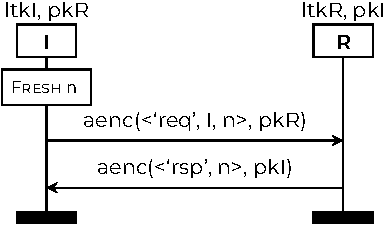
\includegraphics[width=.8\textwidth]
                    {./figures/lecture_8/sources_1}
            \end{figure}
            \begin{itemize}
                \item[] Simple challenge-responder protocol with two messages
            \end{itemize}
        \end{column}
        \begin{column}{.5\textwidth}
            \begin{itemize}
                \item One partial deconstruction (out of six) is caused by 
                      Tamarin failing to find the sources of encryptions
                \item Specifically, Tamarin cannot determine whether the the 
                      \textbf{responder receives a value from the initiator, or 
                      from the attacker}
                \item See Chapter 8.4 in the course book for a detailed 
                      explanation
            \end{itemize}
        \end{column}
    \end{columns}
    \vsep
\end{frame}

\begin{frame}[fragile]{Option 1: Auto-generating sources lemmas}
    \begin{itemize}
        \item Tamarin can automatically try to construct sources lemmas with 
              the command-line argument \verb|--auto-sources|
        \item This will tell Tamarin to look for inputs that cause partial 
              deconstructs and try to solve them
        \begin{itemize}
            \item The algorithm adds action facts \verb|AUTO_IN_| or
                  \verb|AUTO_OUT_| to the rules and creates a sources lemma 
                  using them
        \end{itemize}
        \item Works okay(ish), but is \textbf{not guaranteed to solve the 
                                              problem}
        \item Might produce a lemma that solves the open chains
              \textbf{but cannot be proven}, or one that does not even solve 
              the problem
        \item Use this as a initial option to give you hints for how to solve 
              manually
    \end{itemize}
\end{frame}

\begin{frame}[fragile]{Option 2: Writing sources lemmas manually}
    \begin{itemize}
        \item \textbf{Approach}
        \begin{enumerate}
            \item Identify the rules, messages, and variables causing partial 
                  deconstructions by inspecting the raw sources
            \item For each message input, look for matching outputs
            \item Add additional actions to the rules if needed
            \item Write a lemma proving the potential sources
        \end{enumerate}
        \item If there are multiple partial deconstructions, you have to write 
              lemmas for all of them
        \begin{itemize}
            \item Can also be one large lemma with logical AND (\&) clauses
            \item This is usually easier for Tamarin to prove
        \end{itemize}
    \end{itemize}
\end{frame}

\begin{frame}[fragile,t]{Example}
    \begin{columns}
        \begin{column}{0.5\textwidth}
            \lstinputlisting [
                style = tamarin,
                numbers = left,
                firstline = 23,
                lastline  = 43,
                xleftmargin = .15cm,
            ] {./models/sources.spthy}
        \end{column}
        \begin{column}{0.5\textwidth}
            \lstinputlisting [
                style = tamarin,
                numbers = left,
                firstline = 45,
                lastline  = 55,
                firstnumber = 22,
                xleftmargin = .5cm,
            ] {./models/sources.spthy}
            \vspace*{.25cm}
            \hrule
            \begin{figure}
                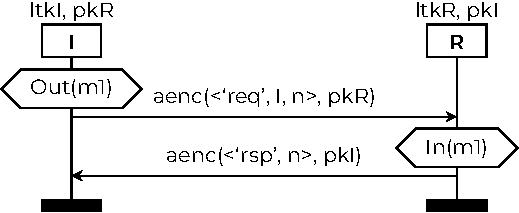
\includegraphics[width=.8\textwidth]{./figures/lecture_8/sources_2}
            \end{figure}
        \end{column}
    \end{columns}
    \vsep
\end{frame}

\begin{frame}[fragile]{Solving paritial deconstructions}
    \begin{itemize}
        \item Intuition: When \verb|Rule_R| receives a message \verb|m| with a 
              variable \verb|x|, then either
        \begin{itemize}
            \item it was the output from \verb|Rule_I_1|, or
            \item the adversary already knew \verb|x| before the message was 
                  received
        \end{itemize}
        \item We can write a lemma stating that
        \begin{enumerate}
            \item either the input was the expected protocol message coming 
                  from the initiator, or
            \item the adversary crafted a message of a corresponding format
        \end{enumerate}
        \item Adding this lemma \textbf{solves the partial deconstruction}
    \end{itemize}
\end{frame}

\begin{frame}[fragile]{Example}
    \textbf{Auto-generated sources lemma:}
        \vspace*{.2cm}
        \begin{lstlisting}[
            style = tamarin,
            gobble = 12,
            mathescape = true,
            xleftmargin = .5cm,
        ]
            lemma AUTO_typing [sources]:
              all-traces
              "($\top$) $\land$
              ($\forall$ x m #i.
              (AUTO_IN_TERM_2_0_0_1_1__Rule_R( m, x ) @ #i) $\Rightarrow$
              (($\exists$ #j. (!KU( x ) @ #j) $\land$ (#j < #i)) $\lor$
               ($\exists$ #j. (AUTO_OUT_TERM_2_0_0_1_1__Rule_R( m ) @ #j) 
               $\land$ (#j<#i))))"
        \end{lstlisting}
    \textbf{Manually written sources lemma:}
        \vspace*{.2cm}
        \lstinputlisting [
            style = tamarin,
            firstline = 57,
            lastline  = 61,
            xleftmargin = .5cm,
        ] {./models/sources.spthy}
\end{frame}

% ---------------------------------------------------------------------------- %

\section{Injective Facts}

% ---------------------------------------------------------------------------- %

\begin{frame}[fragile]{Injective facts}
    \begin{itemize}
        \item Tamarin has built-in support for reasoning about
              injective fact symbols (or \textbf{injective facts} for short),
              i.e., facts whose instances are always \textbf{unique}
        \item An injective fact is one where all instances of the fact
              \texttt{Fact(\tildelow{}x, $\dots$)} come from either an 
              initialization rule that creates it with an actual fresh fact 
              \texttt{Fr(\tildelow{}x)} in its premise, or from a rule that has 
              just consumed and produced it again
        \item Identifying whether a fact symbol is injective is, in general, 
              \textbf{undecidable}
    \end{itemize}
\end{frame}

\begin{frame}[fragile]{Injective facts in Tamarin}
    \begin{itemize}
        \item You can check if Tamarin detected that your theory contains 
              injective facts in the GUI
        \begin{itemize}
            \item To do this, click on \textit{Multiset rewriting rules} on the 
                  left-hand side
        \end{itemize}
        \item Tamarin can \textbf{optimize its reasoning} for facts that it 
              determines to be injective
        \begin{itemize}
            \item When writing models, try to use facts of the form\\
            \begin{center}
                \texttt{Fact(\tildelow{}id, term\_1, term\_2, $\dots$)}\\
            \end{center}
            when e.g., storing state information
        \end{itemize}
    \end{itemize}
\end{frame}

% ---------------------------------------------------------------------------- %

\section{Observational Equivalence}

% ---------------------------------------------------------------------------- %

\begin{frame}[fragile]{Observational equivalence}
    \begin{itemize}
        \item Until now, all properties have been evaluated over individual 
              traces
        \begin{itemize}
            \item These are called \textbf{trace properties} and are ideal for 
                  analyzing security
        \end{itemize}
        \item Observational equivalence describes a hyperproperty that
              \textbf{compares two traces}
        \begin{itemize}
            \item Used to analyze \textbf{privacy properties} like anonymity 
                  and unlinkability
        \end{itemize}
        \item Support in Tamarin was added in 2015~\cite{basin2015obseq}
        \item Concretely: Enter the two systems as a bi-system where one input 
              gives two versions of the same system
        \item The systems are identical, except for terms wrapped under
              \texttt{diff(x,y)}
        \begin{itemize}
            \item \texttt{x} = left instance
            \item \texttt{y} = right instance
        \end{itemize}
    \end{itemize}
\end{frame}

\begin{frame}[fragile]{Differences to trace properties}
    \begin{itemize}
        \item Main difference to trace properties:
              \textbf{No user-defined lemmas}
        \begin{itemize}
            \item Instead: Automatically created equivalence lemma used to 
                  compare two systems
        \end{itemize}
        \item Analyzing the model is similar to the workflow presented in 
              Lecture 6, with some minor changes
        \begin{enumerate}
            \item Fine-tuning heuristics is often less effective
            \begin{itemize}
                \item Instead: Fine-tune the model
            \end{itemize}
            \item Equivalence proofs are often much larger
            \begin{itemize}
                \item Longer verification times
            \end{itemize}
            \item Restrictions cause issues
        \end{enumerate}
    \end{itemize}
\end{frame}

\begin{frame}[fragile]{Use in Tamarin}
    \begin{columns}
        \begin{column}{0.5\textwidth}
            \begin{itemize}
                \item Argument: \verb|--diff|
                \begin{itemize}
                    \item This adds the diff operation to allowed function 
                          symbols and generates extra lemmas
                \end{itemize}
                \item In the \textbf{interactive mode}, Tamarin shows two 
                      versions of the message theory, rules, and precomputed 
                      sources
                \item See Chapter 13 in the course book for examples
            \end{itemize}
        \end{column}
        \begin{column}{0.5\textwidth}
            \begin{lstlisting}[
                style = prooftree,
                gobble = 12,
                mathescape = true,
                xleftmargin = .5cm,
                numbers = none,
            ]
            Diff-Lemmas

            lemma Observational_equivalence:
            rule-equivalence
              case Rule_Alice_and_Bob_pairing
              by sorry
            next
              case Rule_Alice_first
              by sorry
            next
              case Rule_Alice_second
              by sorry
            next
              case Rule_Bob
              by sorry
            next
              case Rule_Destrd_0_fst
              by sorry
            next

              (*@\vdots@*)

            end
            \end{lstlisting}
        \end{column}
    \end{columns}
    \vsep
\end{frame}

% ---------------------------------------------------------------------------- %

\section{User-Specified Equational Theories}

% ---------------------------------------------------------------------------- %

\begin{frame}[fragile]{Recap: Equational theories}
    \begin{itemize}
        \item An \textbf{equational theory} is a set of rules that determine 
              which terms are considered equivalent
        \item \textbf{Motivation:}
        \begin{itemize}
            \item Some messages (such as exponentiation) can be constructed in  
                  more than one way
            \item Convenient for modeling cryptographic primitives
            \item Allows us to model degenerate cases of cryptographic 
                  primitives
        \end{itemize}
    \end{itemize}
\end{frame}

\begin{frame}[fragile]{User-specified equational theories}
    \begin{itemize}
        \item You can define your own equational theories in Tamarin:
        \begin{itemize}
            \item[] \verb|equations: EXPR1 = EXPR2|
        \end{itemize}
        \item For example, we can define symmetric encryption as:
        \begin{itemize}
            \item[] \verb|functions: senc/2, sdec/2|
            \item[] \verb|equations: sdec(senc(m,k),k) = m|
        \end{itemize}
        \item User-defined equational theories
              \textbf{cannot overlap with built-in ones}
        \item Due to fundamental theoretical limitations,
              \textbf{Tamarin cannot handle arbitrary equational theories}
    \end{itemize}
\end{frame}

\begin{frame}[fragile]{Subterm convergence}
    \begin{itemize}
        \item An equation is \textbf{subterm-convergent} when its right-hand 
              side is either a strict subterm of its left-hand side or a 
              constant
        \item An equational theory is subterm-convergent when all of its 
              individual equations have this property
        \begin{itemize}
            \item[] \verb|h(f(X),Y,Z) = f(X)| is subterm-convergent
            \item[] \verb|h(f(X),Y,Z) = f(Y)| is not
        \end{itemize}
        \item An equational theory is supported by Tamarin if:
        \begin{enumerate}
            \item It is subterm-convergent, and
            \item It is syntactically disjoint from the built-in equational 
                  theories
        \end{enumerate}
    \end{itemize}
\end{frame}

\begin{frame}[fragile]{Subterm convergence}
    \begin{itemize}
        \item Equational theories that are \textbf{not subterm-convergent} must 
              at least (1) be convergent, and (2) have the finite variant 
              property (FVP)
        \item This is not trivial to check by users (but still necessary)
        \begin{itemize}
            \item There are tools to help with this
        \end{itemize}
        \item If either condition is not met, Tamarin will almost certainly 
              \textbf{not terminate}
        \item Correctness can also not be guaranteed, since it relies on the 
              correctness of equational theories
    \end{itemize}
\end{frame}

% ---------------------------------------------------------------------------- %
% Reading Material
% ---------------------------------------------------------------------------- %
\begin{frame}[fragile]{Reading material}
    \textbf{Recommended reading}:
        ~\cite[Ch. 8, 13--14]{tamarin-book},
        ~\cite{basin2015obseq}
    \begin{refsection}
        \nocite{tamarin-book,basin2015obseq}
        \printbibliography[heading=none]
    \end{refsection}
\end{frame}

\begin{frame}[fragile]{Reading material}
    \textbf{Additional reading}:
        ~\cite{cryptoeprint:2022/1130},
        ~\cite{dreier2017subterms}
    \begin{refsection}
        \nocite{cryptoeprint:2022/1130,dreier2017subterms}
        \printbibliography[heading=none]
    \end{refsection}
\end{frame}
% ---------------------------------------------------------------------------- %

\end{document}
